% Figure 3 is regenerated by scripts/generate_iclr_figure3_20260829.py.
\begin{figure*}[t]
  \centering
  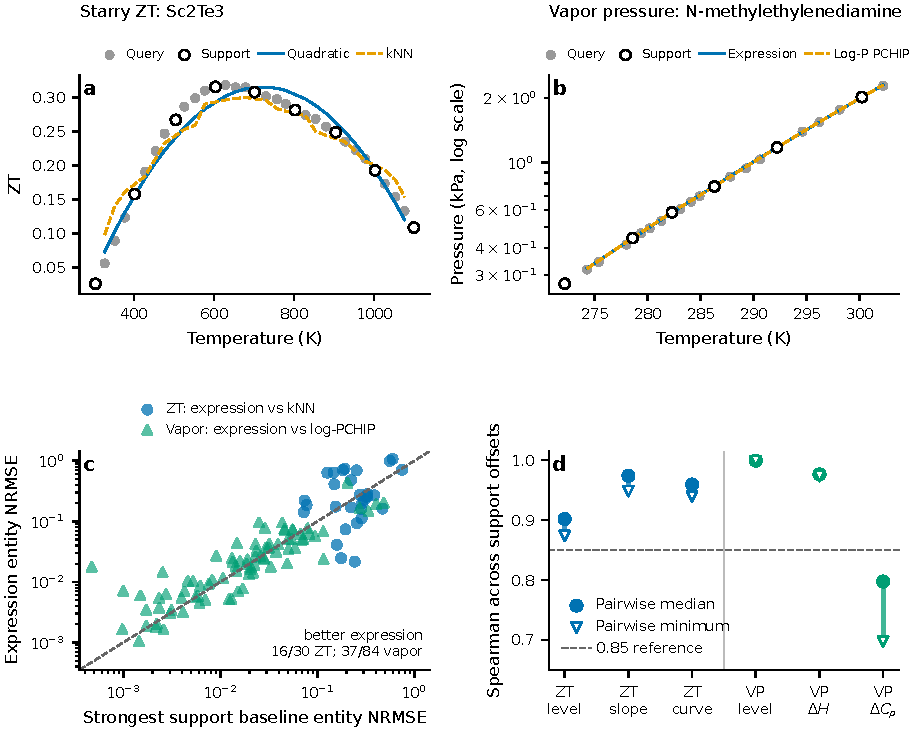
\includegraphics[width=0.90\textwidth]{figures/figure3_real_transfer.pdf}
  \caption{Compact named expressions transfer to unseen future entities, but
  are not uniformly more accurate than local support predictors.
  \textbf{(a,b)} Representative entities are selected mechanically as the
  entity nearest each expression family's median NRMSE, rather than as
  best-case examples.  Black open markers are the only targets available for
  coefficient fitting; gray query targets remain hidden until scoring.
  \textbf{(c)} Paired entity NRMSE against the strongest support-aware baseline;
  points below the diagonal favor the expression.  The expression wins 16/30
  ZT comparisons against kNN and 37/84 vapor-pressure comparisons against
  PCHIP, so pooled fidelity is not predictive superiority.  \textbf{(d)} Median
  (circle) and minimum (triangle)
  pairwise Spearman correlations of named development coefficients over all six
  pairs of four support offsets; the least-stable vapor correction is interpreted
  only as an effective stage-wise term.}
  \label{fig:real-transfer}
\end{figure*}
